\chapter{Spatial Query Orchestration}
As much as it is important to find and save data for the later usage, retrieval of the data in a efficient and logical manner is also a crucial task. It is required that data retrieved from the database in in some logical order. This becomes helpful specially when query result contains large number of output results. User might not look at each and every retrieved data for finding useful information. Most of the time user will use top 5 or 10 entries of the result to make further use. For example, if a user wants to know which are good Chinese restaurants nearby him. A query might select a bounding region and retrieve all the chinese restaurants and show the result to the user. In this case user will not look at each and every restaurants and see their other quality to decide which restaurant he or she wants to go to, rather he will look at merely top 5 restaurants and decide where he wants to go. It is crucial that in this case this top 5 restaurants have some logical qualities that are suitable while retrieving the results. This is where Indexing and ranking of spatial data comes into play, with indexing and ranking of spatial data we can retrieve the useful information from the data in some predefined manner which ranks data into some metrics to gain useful information.

\section{Quadtree based Indexing}
Quad tree is a special kind of tree data structure. In this each node is divided into four child nodes. In node is then either divided into four nodes or kept as it is. Here the leaf nodes cannot be divided further and contains objects and features to be stored in a tree. Geometrically, each node here represents a square, which is further divided into four equal squares. If one cell contains more than one features than it is divided further. If the cell contains one feature only than it becomes leaf node and is not further divided. Quadtrees are highly used in domain such as image processing and spatial indexing. 
\newline
\par Quadtree are specially used for spatial division of data. In this spatial features are drawn on a grid and the quadtree divides the grid such that each of the cell only has one feature in it. Many databases use quadtree for spatial indexing. Indexing can be useful not only in retrieving or select query but also in other type of queries which require data in turn to be executed. 

\subsection{Algorithm}
In this algorithm, quadtree is created based on the number of points and area of indexing also known as bounding box. We first define the bounding box to create a area that defines the points to be inserted. Any points that lie in the bounding box will be added to the tree. Insert all the points into the tree and then select area of intersection. Area of intersection is the area which contains the output features. We can choose different overlap regions to find different features that reside in that area. Accessing the intersection from the quadtree, we can than display various information about the features residing in that area like id, bbox etc.
\begin{algorithm}[h]
    \caption{\em Quadtree Indexing Algorithm }
    \textbf{Input:} Set of spatial point features: features \\
	\textbf{Output:} Arrangement of points when retrieved
	
	\begin{algorithmic}[1]
	    \State $bbox \gets$ set bounding box For $index$
	    \State create $index$ with $bbox$
	    \FOR{ $feature$ in $features$}
	        \State insert $feature$ in $index$
	    \ENDFOR
	    \State $overlap \gets$ select area of interest
	    \State $outputFeatures \gets index.intersect(overlap) $
	    \FOR{$feature$ in $outputFeatures$}
	        \State display $feature$
	    \ENDFOR
	\end{algorithmic}
\end{algorithm}
\subsection{Example Scenario}
Let's look at a example to understand indexing based on a quadtree. Here we take 16 point features in a rectangular region. This points are uniformally distributed over the region in this case, but may not be in the real world. Bounding box for area is (0,0,80,80) and location of the point features are shown in the figure. We can take different overlap regions to find the features which reside in those intersections.
\newline
\begin{figure}[h]
    \centering
    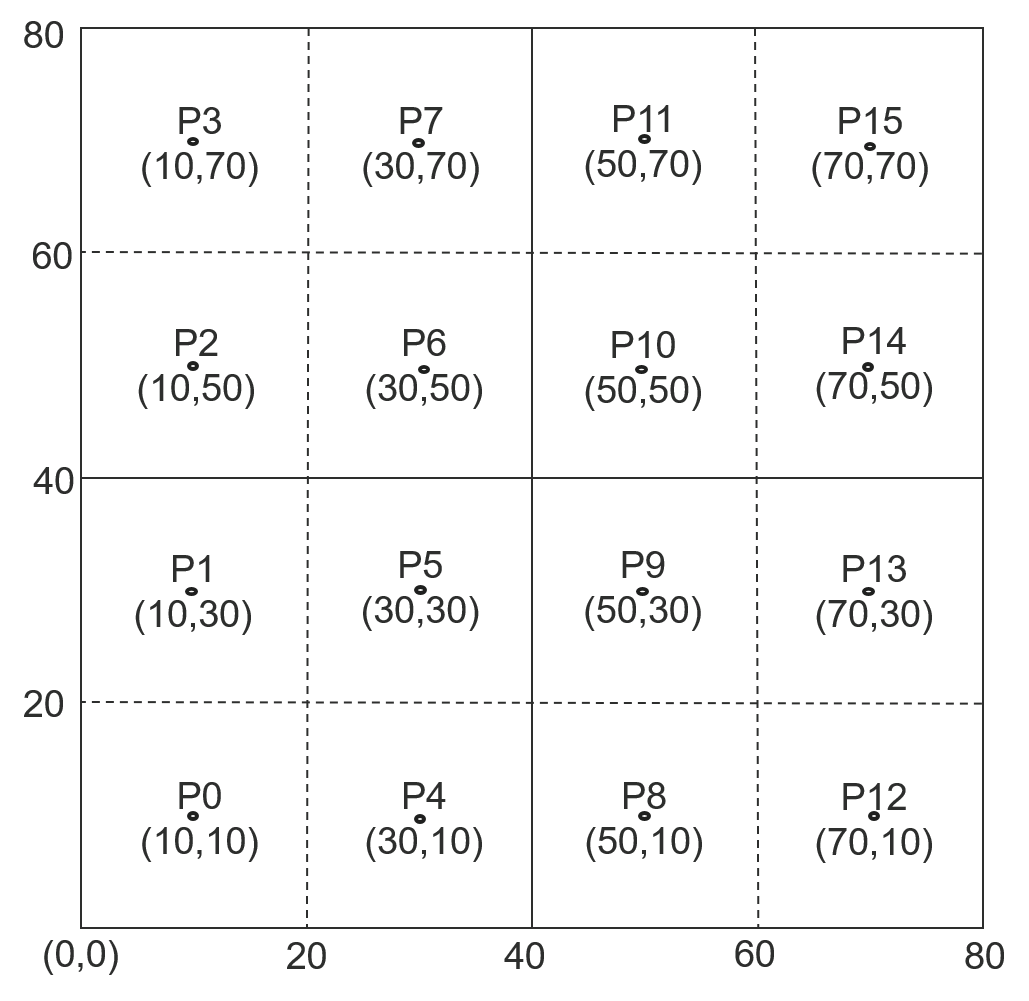
\includegraphics[width=0.7\textwidth]{pix/p10}
    \caption{arrangement of feature points}
    \label{fig:m1}
\end{figure}
\newline
\par Here we take a look at two different intersection regions, $olap1 = (0,20,40,60)$ and $olap2 = (40,20,80,80)$. When we intersect this overlaps with index it gives the points which resides in the intersection as below.

\begin{table}[h]
    \centering
    \begin{tabular}{ |c|c| } 
     \hline
        p2 & (10,50)\\
        \hline
        p1 & (10,30)\\
        \hline
        p6 & (30,50)\\
        \hline
        p5 & (30,30)\\
        \hline
    \end{tabular}
    \caption{Output with overlap region 1}

    \begin{tabular}{|c|c|}
        \hline
        p14 & (70,50)\\
        \hline
        p15 & (70,70)\\
        \hline
        p13 & (70,30)\\
        \hline
        p9  & (50,30)\\
        \hline
        p10 & (50,50)\\
        \hline
        p11 & (50,70)\\
        \hline 
    \end{tabular}
    \caption{Output with overlap region 2}
\end{table}
\par As we can see, quadtree can extract and list features from area of interest.

%-------------------------------------------------------------------------------%
\section{Ranking based on Quality Preferences}

There are other type of advanced ranking mechanism available when more data about the features to be indexed is available. One of such method is ranking based on quality preferences. In this method, we look at some overall mathematical quality of spatial neighbourhood to determine the quality of the feature. There can be more than one methods to rank spatial neighbourhood based on mathematical functions.
\newline
\par For example, If one wants to buy a house, he considers many factors besides the attributes of the house itself. Although qualities of house such as area, no of rooms and price are crucial factors, other neighbourhood qualities such as distance from good quality restaurants or availability of general hospital are also an important factor. One always wants to have his or her home nearby good facilities like hospitals, restaurants and cinemas. The quality of each of this feature in the spatial neighbourhood of house is the determining factor while considering to buy the house.
\newline
\par Quality of each of the facilities is also an important factor. This is why we have defined spatial neighbourhood quality as a parameter of quality of each type of facility and not the quantity of feature types. One can also use the total sum of quality of all features in spatial neighbourhood. That will give the quantitative measure of quality features in the neighbourhood. For example, if there are more number of features that are low in quality, that neighbourhood can still be ranked higher than a spatial neighbourhood where there are less number of high quality features. Other types of mathematical measures can also be employed such as average quality of each feature or sum of average quality of each feature type in spatial neighbourhood. 

\subsection{Algorithm}
This algorithm ranks the quality of spatial neighbourhood for every feature to be ranked. Set of input features with information about other qualitative features are required for this purpose. We also need to set neighbourhood radius for examining spatial neighbourhood. The algorithm takes the input and finds the ranking of the input features. To do this, it first scans the spatial neighbourhood around each features. This is done by creating a bounding box of specified radius around the feature point. We find all the qualitative features in the spatial neighbourhood and find the maximum quality of each type of feature from the neighbourhood. The sum of each type of quality feature gives a score to a particular input feature. Input feature are ranked by decreasing order of their neighbourhood score.
\newline
\begin{algorithm}[h]
    \caption{\em Ranking based on quality preferences }
    \textbf{Input:}\\
    \indent \textit{features}: Set of spatial point features  \\
    \hspace{1cm} \textit{qualitative\_features}: Set of features with quality\\
    \textit{radius}: Spatial neighbourhood radius\\
	\textbf{Output:}\\ 
	\hspace{1cm} Ranking of input features based quality of spatial neighbourhood
	
	\algnewcommand{\Initialize}[1]{%
        \State \textbf{Initialize:}
        \Statex \hspace*{\algorithmicindent}\parbox[t]{.8\linewidth}{\raggedright #1}
        \newline
    } 
	
	\begin{algorithmic}[1]
	    \Initialize{
	        \State $boundary\_box \gets $ Create bounding box based on radius and feature bounding box
	        
	    }
	    \FOR{$feature$ in $features$}
	        \State $qfeatures \gets $ Get all $qualitative\_features$ in the $boundary\_box$ of $feature$
	        \State $feature.quality \gets 0$
	        \FOR{$qtype$ in $qualitative\_feature$ types}
	            \State $qtype.quality \gets$ extract maximum quality for the $type$ in $bondary\_box$
	            \State $feature.quality \gets feature.quality + qtype.quality $
	        \ENDFOR
	    \ENDFOR
	    \State $ranked\_list \gets features$ ranked by $feature.quality$
	    \FOR{$feature$ in $ranked\_list$}
	        \State $Display(feature)$
	    \ENDFOR
	\end{algorithmic}
\end{algorithm}

\subsection{Example Scenario}
\par In our example, we have taken four feature points to rank. They are $feature0(20,20)$, $feature1(20,60)$, $feature2(60,20)$ and $feature3(60,60)$. There are two types of neighbourhood features that we are interested in called box features and star features. Locations of star features are x1(10,70), x2(30,70), x3(10,30), x4(30,30), x5(10,10) and x6(50,30). Locations of box features are y1(10,50), y2(50,70), y3(70,70), y4(70,50), y5(70,30), y6(70,10). Quality of each box and star features are shown in the figure \ref{figure:quality_ranking}.
\newline
\begin{figure}[h]
    \centering
    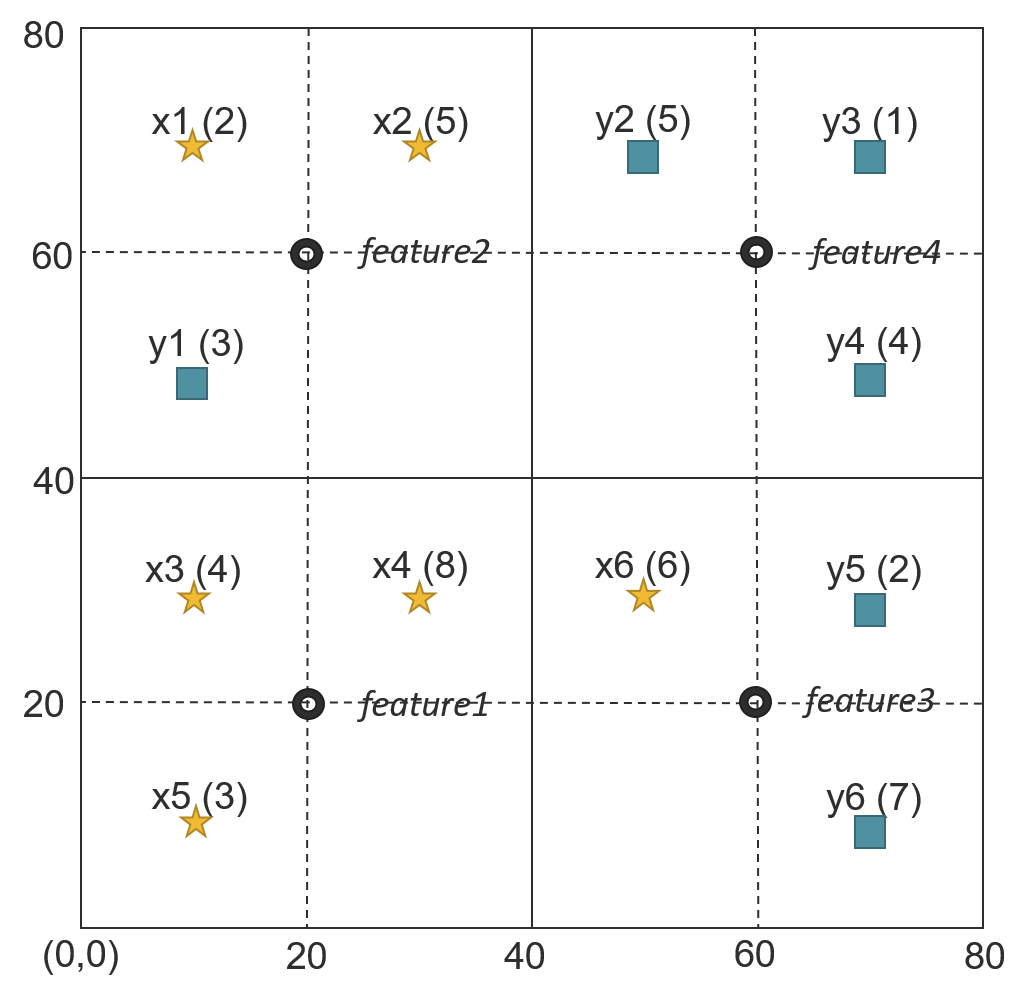
\includegraphics[width=0.7\textwidth]{pix/p11}
    \caption{Ranking by quality preferences}
    \label{figure:quality_ranking}
\end{figure}
\newline
\par In this approach, we first iterate on the feature points, here $feature1, feature2, feature3$ and $feature4$. For each feature we take a neighbourhood region corresponding to it. Here we have taken neighbourhood region to be of 20 distance buffer from the feature point. We find all the relevant features from this buffer and we find maximum quality of star feature and maximum quality of box feature from this buffer. This selected features represents the buffer and in transitive manner the feature itself. We can apply various operations to determine the quality of spatial neighbourhood by applying various mathematical functions on top of it. Here we have chosen the sum function for the demonstrative purposes.
\newline
\par For each feature, the sum of other qualitative features in neighbourhood gives the final score of a feature. The higher the score, lesser the rank. In this example, our final ranking becomes.
\begin{table}[h]
    \centering
    \begin{tabular}{|c|c|}
        \hline
         $Feature$&$Rank$\\
         \hline
         2&13\\
         \hline
         0 & 8 \\
         \hline
         1 & 8\\
         \hline
         3 & 5\\
         \hline
    \end{tabular}
    \caption{Final ranking for the features}
    \label{tab:my_label}
\end{table}
\newline
\begin{figure}[h]
    \centering
    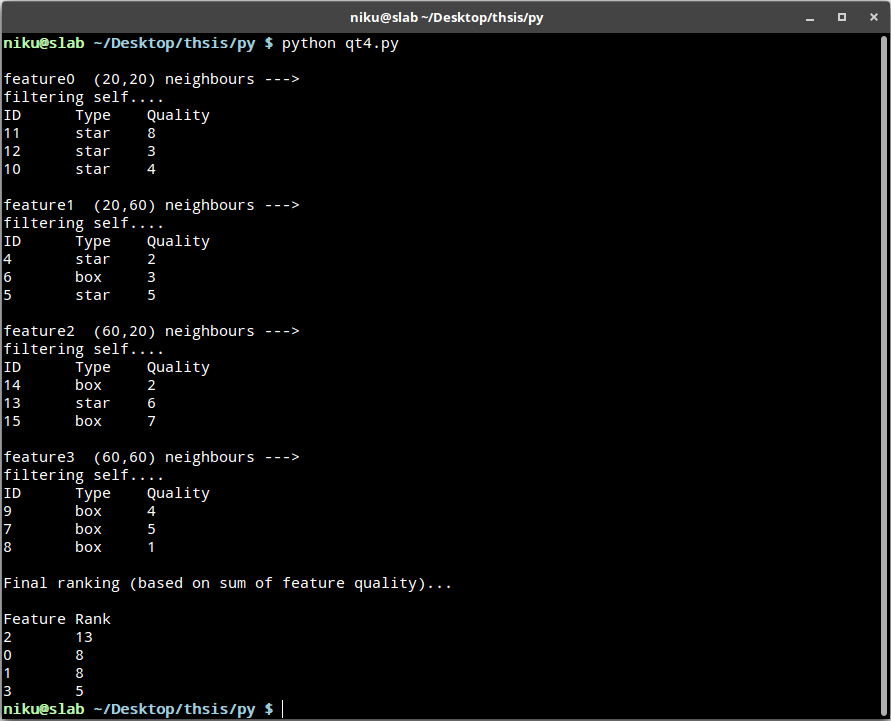
\includegraphics[width=\textwidth]{pix/p12}
    \caption{Features ranked by neighbourhood quality}
    \label{feature_ranking}
\end{figure}
\newline

